\documentclass{article}

\PassOptionsToPackage{numbers,sort&compress}{natbib}
\usepackage{nips_2016}

\usepackage[utf8]{inputenc}
\usepackage[T1]{fontenc}
\usepackage{hyperref}
\usepackage{url}
\usepackage{booktabs}
\usepackage{amsfonts}
\usepackage{nicefrac}
\usepackage{microtype}
\usepackage{graphicx}
\usepackage{multirow}
\usepackage{array}
\usepackage{enumitem}
\usepackage{float}
\usepackage{newunicodechar}
\newunicodechar{↳}{$\hookrightarrow$}

\title{Cross-Cultural Music Representation Learning with Deep Audio Models}

\author{
 Bin Zhou \\
 KTH Royal Institute of Technology \\
 \texttt{bzhou@kth.se}
 \And
 Jiahang Lyu \\
 KTH Royal Institute of Technology \\
 \texttt{jiahang@kth.se}
}

\makeatletter
\renewcommand{\@noticestring}{}
\makeatother

\begin{document}

\maketitle

\begin{abstract}
Music foundation models achieve strong results on Music Information Retrieval (MIR) tasks, but their benchmarks and pretraining corpora are dominated by Western music, leaving their cross-cultural generalization unclear. We study this question with MERT, a large-scale music foundation model, by constructing a balanced 18-genre dataset that spans Western and Eastern traditional and modern styles. Across baseline classification, cross-cultural transfer, multi-task learning, confusion-aware hard mining, and layer-wise probing, we find that MERT separates traditional genres well but represents modern popular genres from different regions with substantial overlap. Transferring Western-trained classifiers to Eastern music causes clear negative transfer, and layer-wise analysis shows that MERT's mid-to-deep layers are shaped by Western musical structure. t-SNE and confusion-matrix visualizations corroborate these findings. Overall, current music foundation models still encode meaningful cultural biases, underscoring the need for culturally diverse training corpora and benchmarks.
\end{abstract}

\section{Introduction}

Recent years have witnessed rapid progress in foundation models for music representation learning. Large-scale pretrained models such as MusicLM~\cite{agostinelli2023musiclm}, MuLan~\cite{huang2022mulan}, and MERT~\cite{li2024mert} have significantly improved performance across a wide range of Music Information Retrieval (MIR) tasks~\cite{humphrey2013feature, lee2009unsupervised, van2013deep}, including genre classification, tagging, retrieval, and music understanding. However, previous MIR research has primarily focused on Western datasets such as GTZAN~\cite{tzanetakis2002musical} and FMA~\cite{defferrard2016fma}, while cross-cultural music understanding remains relatively underexplored.

At the same time, globalization and industrialized music production have caused modern popular music genres from different regions to become increasingly similar in timbre and production style. In contrast, many traditional music genres still preserve strong regional and cultural uniqueness. This raises an interesting representation learning question: how do foundation music models organize traditional and modern music from different cultures in latent space?

To investigate this problem, we construct a unified cross-cultural music dataset of Western and Eastern genres---traditional and modern styles from China, Japan, Korea, India, and the West---and, using representations extracted from MERT, conduct baseline genre classification, cross-cultural transfer learning, multi-task learning, confusion-aware hard mining, and layer-wise representation analysis.

Our main contributions are as follows:
\begin{itemize}[leftmargin=*]
 \item We construct a unified cross-cultural music dataset of 18 Western and Eastern genres.

 \item We systematically analyze how MERT represents culturally distinct music through classification, transfer learning, and layer-wise probing.

 \item We show that traditional genres remain highly separable in latent space while modern popular music converges across cultures, and that Western-trained representations transfer negatively to Eastern music.
\end{itemize}

\section{Dataset Construction}
\subsection{Dataset Collecting}

A major limitation in cross-cultural MIR research is the lack of a unified benchmark containing both Western and Eastern music genres. To address this issue, we construct a cross-cultural music dataset containing 18 genres from Western and Eastern music traditions, where the Eastern subset spans four cultural regions (Table~\ref{tab:dataset}).

The Western subset is mainly derived from the GTZAN dataset~\cite{tzanetakis2002musical}, while the Carnatic genre is collected from a public Carnatic music dataset~\cite{krishnan2025sanidha}. The remaining Eastern genres are collected from Bilibili, where we manually selected high-quality and genre-consistent recordings. Only videos marked as reprintable or openly reusable were included to ensure ethical compliance for academic research. The dataset intentionally mixes culturally distinctive traditional genres---Classical, Carnatic, Sitar, Guzheng/Guqin, Jingju, and Enka---with globally influenced modern popular genres, so that cultural separability can be studied across both categories.
\begin{table}[h]
\centering
\caption{Cross-cultural music dataset: 18 genres from Western and Eastern music traditions, where the Eastern subset spans four cultural regions.}
\label{tab:dataset}
\small
\begin{tabular}{l l c @{\hspace{2.5em}} l l c}
\toprule
\textbf{Genre} & \textbf{Region} & \textbf{Samples} & \textbf{Genre} & \textbf{Region} & \textbf{Samples} \\
\midrule
Blues & Western & 100 & Carnatic & India & 100 \\
Classical & Western & 100 & Sitar & India & 55 \\
Country & Western & 100 & Guzheng/Guqin & China & 100 \\
Disco & Western & 100 & Jingju & China & 100 \\
Hiphop & Western & 100 & C-pop & China & 100 \\
Jazz & Western & 100 & Enka & Japan & 39 \\
Metal & Western & 100 & J-pop & Japan & 68 \\
Pop & Western & 100 & K-pop & Korea & 100 \\
Reggae & Western & 100 & & & \\
Rock & Western & 100 & & & \\
\bottomrule
\end{tabular}
\end{table}
\subsection{Preprocessing and Leakage-Aware Splitting}

All tracks are resampled to 24~kHz and segmented into 30-second audio slices~\cite{mcfee2015librosa} to increase training diversity. We use a 60\% / 20\% / 20\% train / validation / test split and adopt a strict two-level leakage protection.
First, slice-level leakage is prevented by splitting at the track level so that
no two slices from the same recording appear in different subsets. Second, \emph{artist-level leakage} is prevented through group-aware splitting: for the Western subset, we use the manually curated artist and song index released by
Sturm~\cite{sturm2013gtzan}\footnote{\url{https://github.com/boblsturm/GTZAN}} to assign each GTZAN file to an (artist, song) group, so that all recordings by the same artist---and any cross-genre song duplicates---are confined to a single split. For the Eastern subset, each recording is assigned a source identifier derived from its origin playlist or uploader; recordings sharing a source identifier are kept in the same split. All evaluation is performed using stratified group $k$-fold cross-validation (\texttt{StratifiedGroupKFold}, $k = 5$), which simultaneously balances class distribution and prevents group bleeding across folds.

We note that prior work routinely overlooks artist-level leakage on GTZAN, leading to inflated accuracies; Flexer~\cite{flexer2007closer} reports that introducing artist filters typically reduces reported accuracies by 5--15 percentage points. Our results below are reported under the leakage-safe protocol throughout.

\section{Method}
\begin{figure}
 \centering
 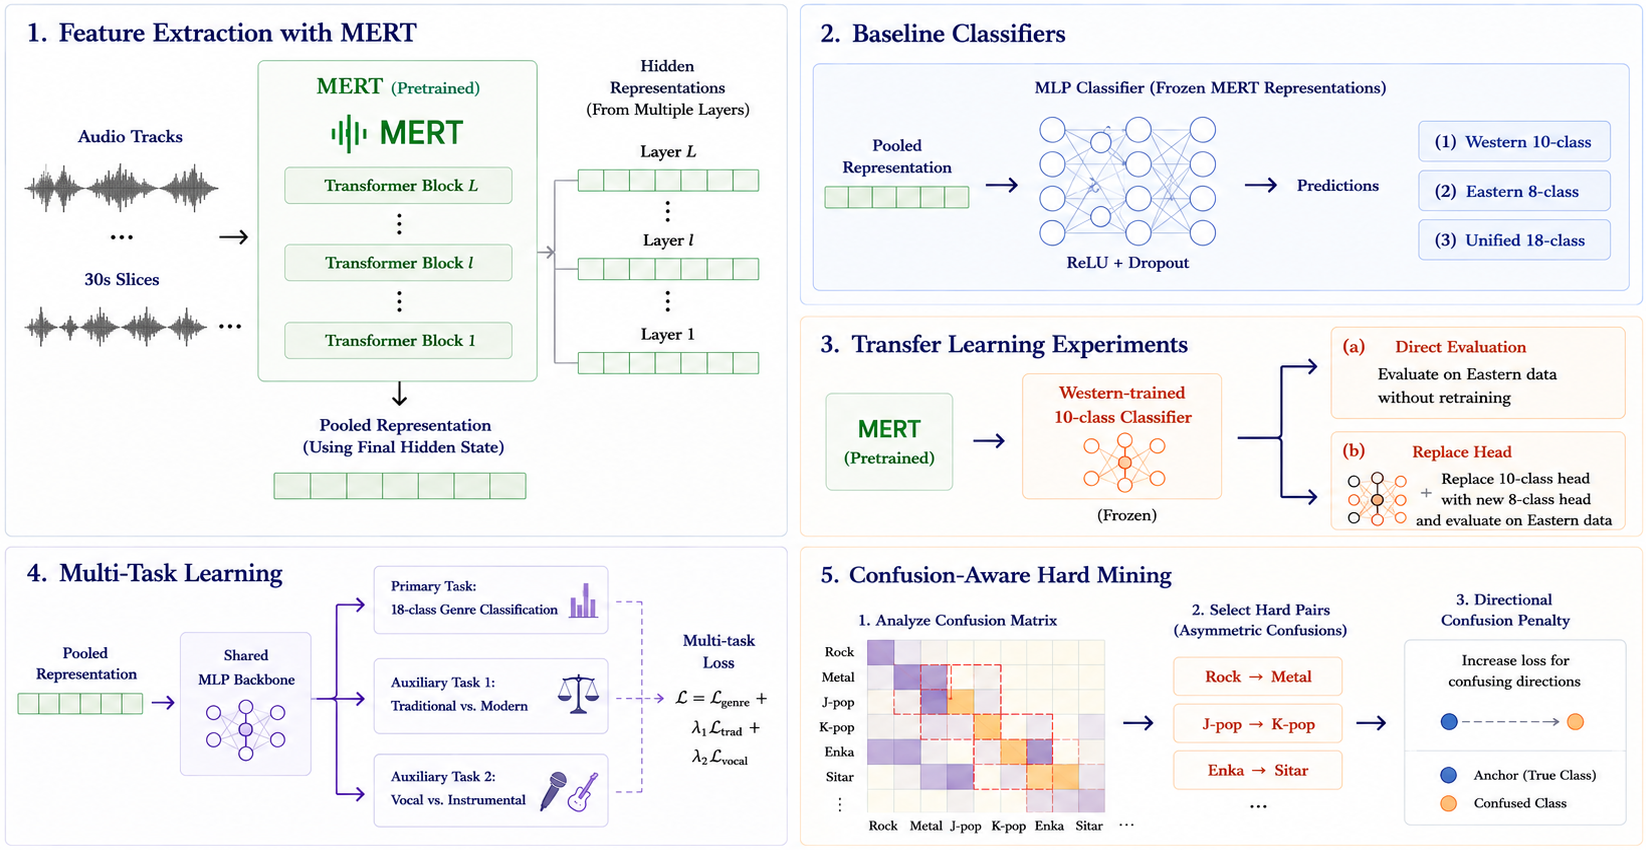
\includegraphics[width=1.0\linewidth]{method.png}
 \caption{Overview of the experimental methodology. Audio is segmented into
 30-second slices and encoded by a frozen MERT model; lightweight downstream
 modules then perform baseline classification, cross-cultural transfer,
 multi-task learning, confusion-aware hard mining, and layer-wise probing.}
 \label{fig:method}
\end{figure}

\subsection{Feature Extraction with MERT}

We use MERT~\cite{li2024mert} as the backbone representation extractor as shown in Figure~\ref{fig:method}. Audio slices are processed through the pretrained transformer encoder, and hidden representations are extracted from its transformer layers; the exact layers used in each experiment are specified in Section~4.1.

\subsection{Baseline Classifiers}
We first establish three baseline tasks: Western 10-class genre classification; Eastern 8-class genre classification; Unified 18-class cross-cultural classification.

A lightweight multilayer perceptron (MLP) classifier is trained on top of frozen MERT~\cite{li2024mert} representations. The classifier consists of fully connected layers with ReLU activations and dropout regularization.

\subsection{Transfer Learning Experiments}

To investigate cross-cultural transferability~\cite{pan2009survey, choi2017transfer}, we perform two transfer learning experiments.

First, we directly evaluate a Western-trained classifier on Eastern music samples without retraining. Second, we reuse the learned Western classifier while replacing the final 10-class prediction head with a new Eastern classification head.

\subsection{Multi-Task Learning}

We further investigate whether introducing external semantic knowledge improves cross-cultural classification. Besides the primary 18-class genre classification task, we introduce two auxiliary tasks~\cite{ruder2017overview}: traditional versus modern music classification and vocal versus instrumental classification. These auxiliary objectives encourage the latent representation to capture higher-level semantic organization beyond individual genres.

\subsection{Confusion-Aware Hard Mining}

Analysis of confusion matrices~\cite{susmaga2004confusion} reveals several consistently ambiguous genre pairs. To address these ambiguities, we introduce a lightweight confusion-aware hard mining strategy that increases the loss contribution of predefined difficult confusion directions.

Unlike symmetric metric learning objectives, our approach uses directional confusion penalties, reflecting the observation that genre confusion is often asymmetric.

\section{Experiments}

\subsection{Experimental Setup}

All experiments are conducted using frozen MERT-v1-95M~\cite{li2024mert} representations with lightweight downstream classifiers implemented in PyTorch. Audio is processed at 24~kHz; for each 30-second slice we extract the hidden states from all 12 transformer layers and apply mean pooling over the time dimension, yielding one 768-dimensional vector per layer per slice. For the main classification experiments we use the final-layer representation; for the layer-wise probing experiment we use representations from each individual transformer layer.

We use \texttt{StratifiedGroupKFold} with $k=5$ (random seed $42$) so that each fold respects both class balance and the group constraints described in Section~2.2. Within each fold, training tracks are used for parameter fitting, validation tracks for early stopping, and test tracks for the final evaluation. We report the mean and standard deviation across the five test folds.

Track-level prediction is obtained by soft voting: slice-level posterior probabilities are averaged within a track and the maximum aggregated probability determines the final label. Because the dataset is moderately imbalanced, macro-F1 is used as the primary evaluation metric.

\subsection{Experimental Detail}

\paragraph{MLP classifier.}
The downstream classifier is a two-layer multilayer perceptron operating on
the 768-dimensional MERT representation. The architecture is
$\mathrm{Linear}(768 \!\to\! 64) \to \mathrm{ReLU} \to \mathrm{Dropout}(p\!=\!0.5)
\to \mathrm{Linear}(64 \!\to\! C)$, where $C$ is the number of target classes
($10$, $8$, or $18$ depending on the task).

\paragraph{Training configuration.}
Models are optimized with AdamW (learning rate $3\times 10^{-4}$, weight
decay $1\times 10^{-3}$). We use cross-entropy loss with label smoothing
$0.05$ and apply class-weighted sampling proportional to inverse class
frequency to mitigate the imbalance among Eastern genres. Each model is
trained with early stopping on validation macro-F1
(patience $5$). Batch size is $32$.
After cross-validation, a final model is trained on the union of training
and validation tracks for the median best epoch across folds.

\paragraph{Transfer learning.}
The \emph{direct evaluation} setting feeds Eastern features through the
Western-trained MLP without any retraining; predictions are recorded as
projections onto the Western 10-class label space, and we report the
projection distribution, mean confidence, and predictive entropy (the
labels are non-overlapping, so accuracy is undefined). The
\emph{head replacement} setting freezes the hidden layer of the
Western-trained MLP and re-initializes only the final classification
layer, which is then trained on the Eastern training split with the
same optimizer and stopping criterion as the baseline.

\paragraph{Multi-task learning.}
The multi-task model shares the MLP hidden layer across three heads
operating on the unified 18-class data: the primary genre head, a binary
\emph{traditional vs.\ modern} head, and a binary \emph{vocal vs.\
instrumental} head. Auxiliary labels are deterministically assigned per
genre using a manually curated mapping (e.g.\ Guzheng/Guqin and Sitar are
labelled instrumental-traditional; K-pop and Western Pop are
vocal-modern). The total loss is
$\mathcal{L} = \mathcal{L}_{\mathrm{genre}} + \lambda_1\,\mathcal{L}_{\mathrm{trad}}
+ \lambda_2\,\mathcal{L}_{\mathrm{vocal}}$ with
$\lambda_1 = \lambda_2 = 0.2$.

\paragraph{Confusion-aware hard mining.}
Following an analysis of the baseline 18-class confusion matrix, we manually identify
asymmetric confusion pairs that repeatedly appear as directional errors. For an
anchor sample of true class $a$ that is at risk of being confused with class $b$,
we multiply its per-sample cross-entropy loss by a factor
$1 + p(b \mid x)(\gamma - 1)$, where $\gamma=2.0$ is the hard-mining weight. The set of mined pairs includes
\emph{Enka $\to$ Sitar}, \emph{C-pop $\to$ Enka}, and \emph{Rock $\to$ Metal},
among others. The penalty is asymmetric: only the specified directions
are penalized.

\paragraph{Layer-wise probing.}
To diagnose which transformer depth carries the most genre-discriminative
information, we train an independent linear probe on the pooled output of
each of the 12 transformer layers. The probe is a multinomial logistic
regression (\texttt{scikit-learn}, $C\!=\!1.0$, \texttt{class\_weight=balanced},
\texttt{lbfgs} solver, max $2000$ iterations); features are standardized using
statistics computed only on the training split of each fold. We deliberately
use a linear probe rather than the MLP head so that the reported numbers
reflect the linear separability of each layer's raw representation.


\subsection{Evaluation Metrics}

We report accuracy and macro-F1, with macro-F1 as the primary metric since it better reflects performance across both majority and minority genres.

To better understand the latent geometry learned by MERT~\cite{li2024mert}, we visualize pooled representations using t-SNE dimensionality reduction~\cite{maaten2008visualizing} and analyze normalized confusion matrices to investigate genre-level ambiguities and cultural overlap. These visualizations are used as qualitative evidence rather than as standalone quantitative metrics.

\section{Results}

\subsection{Baseline Classification}
\begin{table}[h]
\centering
\caption{Baseline classification under leakage-safe (artist- and
source-grouped) 5-fold cross-validation. ``Western subset'' and
``Eastern subset'' rows decompose the 18-class result by region.}
\label{tab:baselines}
\small
\begin{tabular}{lcc}
\toprule
\textbf{Setting} & \textbf{Test Accuracy} & \textbf{Test Macro-F1} \\
\midrule
Western 10-class & $0.6249 \pm 0.0571$ & $0.5886 \pm 0.0531$ \\
Eastern 8-class  & $0.9086 \pm 0.0250$ & $0.8366 \pm 0.0391$ \\
Unified 18-class & $0.7791 \pm 0.0181$ & $0.6502 \pm 0.0213$ \\
\quad ↳ Western subset only & --- & $0.5913$ \\
\quad ↳ Eastern subset only & --- & $0.7709$ \\
\bottomrule
\end{tabular}
\end{table}
Table~\ref{tab:baselines} summarizes the performance of the three baseline classifiers under the leakage-safe evaluation protocol. Two observations can be made. First, the Western 10-class classifier achieves $58.86\%$ macro-F1, which is lower than frequently reported results on GTZAN and is consistent with previous observations regarding potential evaluation bias in music genre classification~\citep{flexer2007closer}. Second, the Eastern 8-class classifier achieves substantially higher performance ($83.66\%$ macro-F1) under the same backbone and classifier setting.

The unified 18-class classifier reaches $65.02\%$ macro-F1. When decomposed by region, the Western subset achieves $59.13\%$ macro-F1 and the Eastern subset achieves $77.09\%$, indicating that the performance difference between the two subsets remains present under joint training.

\subsection{Negative Transfer Effects}

Both transfer learning experiments~\citep{pan2009survey,choi2017transfer} exhibit negative transfer behavior. Directly applying a Western-trained classifier to Eastern music severely distorts the original latent-space clustering structure as shown in Figure~\ref{fig:experiment1_tsne}. Furthermore, reusing the Western-learned representation while retraining only the classification head does not recover the baseline performance, with macro-F1 decreasing from $83.66\%$ to $52.22\%$. These results indicate limited transferability of Western-trained representations to Eastern music classification.

\subsection{Multi-Task Learning and Hard Mining}
\begin{table}[h]
\centering
\caption{Ablation study on improving the unified 18-class cross-cultural classifier. Results are reported using track-level evaluation with soft voting across slices.}
\label{tab:ablation}
\small
\begin{tabular}{lcccc}
\toprule
\textbf{Method} & \textbf{Test Accuracy} & \textbf{Test Macro-F1} \\
\midrule
Baseline & 0.7791 & 0.6502 \\

Multi-task only & \textbf{0.8720} & \textbf{0.8189} \\

Hard Mining only & 0.8640 & 0.8118 \\

Full Model (Multi-task + Hard Mining) & 0.8592 & 0.8055 \\
\bottomrule
\end{tabular}
\end{table}
As shown in Table~\ref{tab:ablation}, both multi-task learning~\citep{ruder2017overview} and confusion-aware hard mining~\citep{susmaga2004confusion} improve performance over the baseline model. Multi-task learning achieves the largest improvement, while hard mining also provides measurable gains.

Combining both methods does not further improve performance. Possible explanations for this observation are discussed in Section~6.

\subsection{Layer-Wise Representation}

\begin{figure}[h]
 \centering
 \begin{minipage}{0.49\linewidth}
   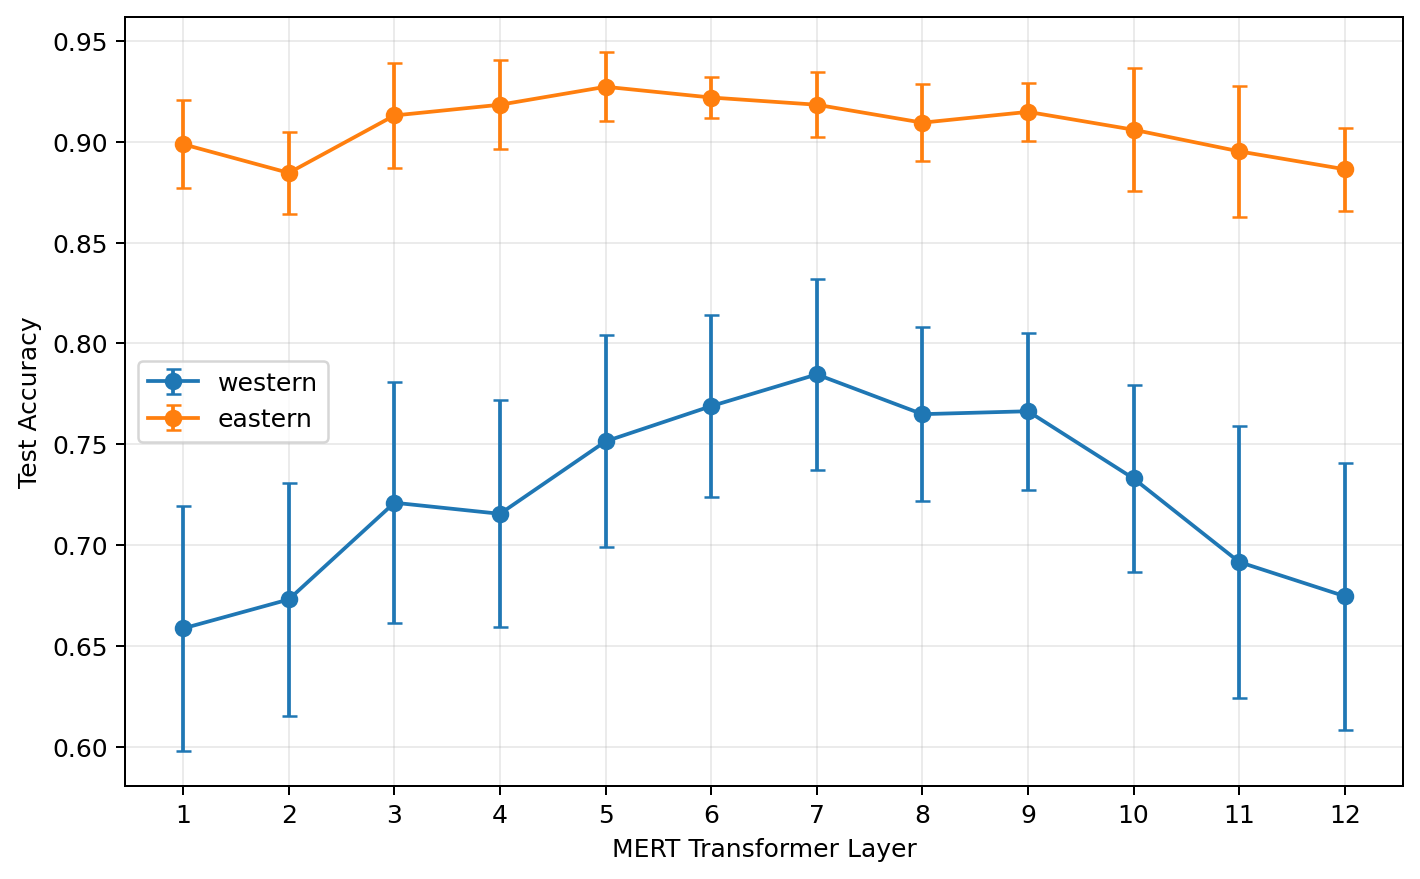
\includegraphics[width=\linewidth]{accuracy_curve.png}
 \end{minipage}
 \begin{minipage}{0.49\linewidth}
   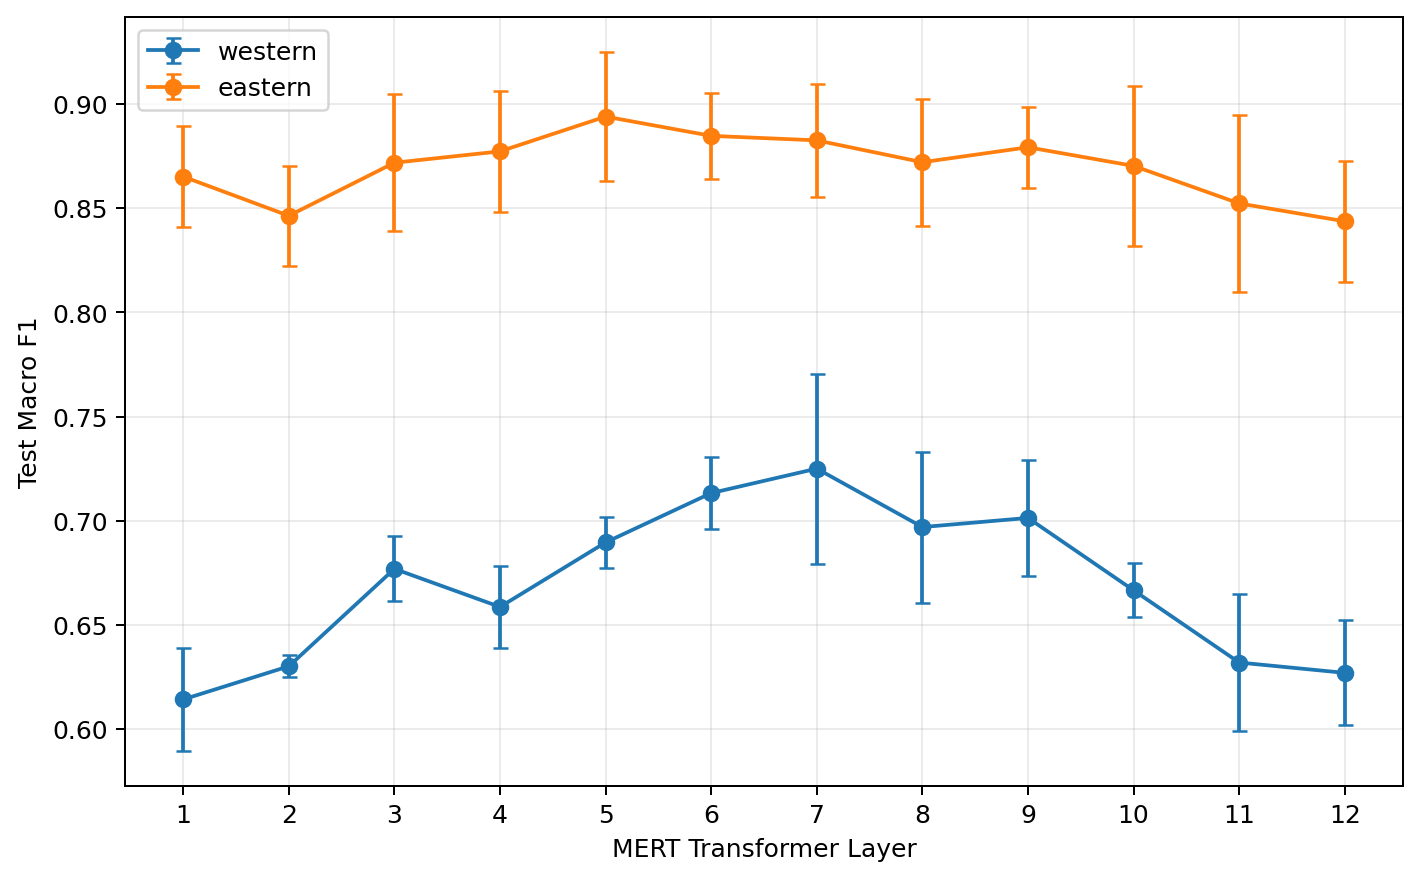
\includegraphics[width=\linewidth]{macro_f1_curve.png}
 \end{minipage}
 \caption{Linear-probe performance at each MERT transformer layer.
 Left: test accuracy. Right: test macro-F1. Error bars denote the
 standard deviation across 5 leakage-safe folds. The Western curve
 peaks at layer~7 and declines at layers~11--12, whereas the Eastern
 curve is near-saturated from layer~1.}
 \label{fig:layerwise}
\end{figure}

Figure~\ref{fig:layerwise} shows that different MERT layers exhibit different discriminative abilities across the two classification tasks. For Western genres, performance increases from shallow to middle layers and reaches its maximum around the middle transformer layers before decreasing in deeper layers. In contrast, Eastern genres achieve relatively strong performance even in shallow layers, with only limited variation across layers.

These results suggest differences in how the learned representation hierarchy contributes to the two classification settings.

\subsection{Visualization Findings}
\begin{figure}[h]
 \centering
 \begin{minipage}{0.49\linewidth}
   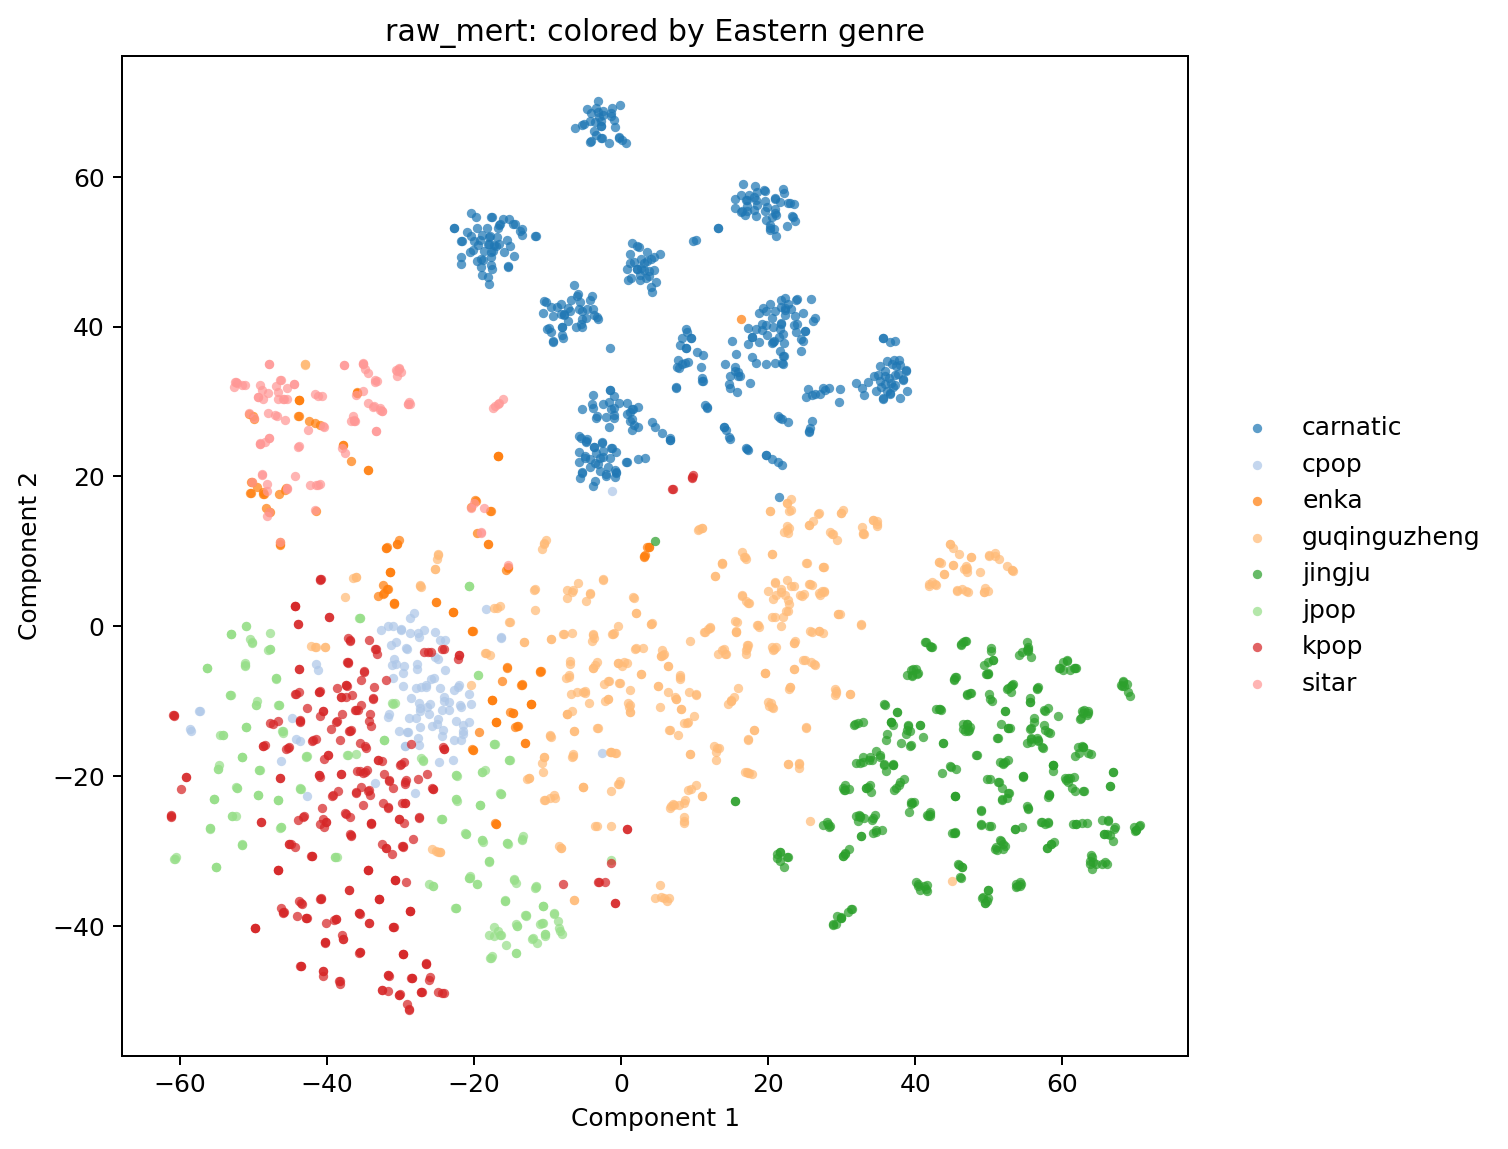
\includegraphics[width=\linewidth]{raw_mert_tsne_by_eastern_genre.png}
 \end{minipage}
 \begin{minipage}{0.49\linewidth}
   
\includegraphics[width=\linewidth]{mlp_penultimate_tsne_by_eastern_genre.png}
 \end{minipage}
 \caption{t-SNE visualization of Eastern music in the Western-bias probing experiment. Left: raw MERT feature space. Right: penultimate features after the Western-trained MLP.}
 \label{fig:experiment1_tsne}
\end{figure}

\begin{figure}[h]
 \centering
 \begin{minipage}{0.49\linewidth}
   
\includegraphics[width=\linewidth]{confusion_matrix_normalized.png}
 \end{minipage}
 \begin{minipage}{0.49\linewidth}
   
\includegraphics[width=\linewidth]{region_confusion_matrix.png}
 \end{minipage}
 \caption{Confusion analysis of the unified 18-class classifier. Left: row-normalized genre-level confusion matrix. Right: region-level confusion matrix.}
 \label{fig:confusion}
\end{figure}

Figure~\ref{fig:confusion} presents confusion analysis of the learned representations. Traditional genres such as Guqin/Guzheng, Jingju, Carnatic, and Sitar exhibit relatively strong separability, whereas modern genres such as C-pop, J-pop, and K-pop show stronger overlap.

For the Western-trained classifier applied to Eastern samples, modern Eastern genres are predominantly assigned to Western popular genres, while traditional Eastern genres are more frequently mapped to Western classical categories.

For the unified 18-class classifier, the normalized confusion matrix shows that classification errors are not uniformly distributed across genres. Traditional genres remain relatively separable, whereas stronger mutual confusion is observed among modern genres. The region-level confusion matrix additionally indicates that most errors occur within similar cultural or production-style groups.

Overall, the visualization results are consistent with the quantitative findings presented in previous sections.


\section{Discussion}

\paragraph{Negative transfer and cultural bias.}
The transfer learning experiments reveal clear negative transfer effects when Western-trained representations are reused for Eastern music classification~\citep{pan2009survey,choi2017transfer}. Although MERT is pretrained on large-scale music corpora~\citep{li2024mert}, the learned latent space does not appear to be fully culture-invariant. Visualization results further support this observation, showing stronger overlap among modern genres while traditional genres remain relatively separable.

\paragraph{Effect of auxiliary learning strategies.}
The ablation experiments show that multi-task learning~\citep{ruder2017overview} and confusion-aware hard mining~\citep{susmaga2004confusion} provide measurable improvements but do not fundamentally alter the learned representation structure. Their limited combined effect may indicate partially overlapping supervision signals rather than complementary information. For example, emphasizing difficult pairs such as Enka--Sitar through hard mining may implicitly encourage the model to distinguish vocal and instrumental characteristics, which resembles the role of the vocal-versus-instrumental auxiliary task. Similarly, emphasizing Enka--C-pop confusion may partially align with the traditional-versus-modern auxiliary supervision. These examples suggest that both approaches may guide the model toward similar latent separations, thereby limiting additional gains when combined.

\paragraph{Cross-cultural representation differences.}
The experimental results suggest that performance differences across Western and Eastern classification tasks should not be interpreted purely as stronger semantic understanding. The layer-wise analysis shows that Eastern genres achieve relatively strong performance even in shallow MERT layers, whereas Western genres benefit more from middle-layer representations, suggesting that the two settings rely on different levels of information within the learned representation hierarchy.

The visualization results further show that traditional genres remain relatively well separated, whereas stronger overlap is observed among modern genres. This suggests that traditional music preserves stronger culturally distinctive characteristics, while modern genres across regions increasingly share similar latent structures.

\paragraph{Limitations.}
Several limitations should be acknowledged. First, although the proposed dataset combines multiple sources, its scale remains relatively small compared with modern music benchmarks and contains moderate class imbalance for several genres. Second, the subset covers only a limited number of cultural traditions and excludes many important musical systems from regions such as Africa, the Middle East, and Southeast Asia.

\paragraph{Future work.}
Future research may investigate larger and more culturally balanced datasets, culturally adaptive pretraining strategies, and self-supervised objectives specifically designed for cross-cultural music understanding. Incorporating music-theoretic knowledge, including rhythmic structures, tonal systems, instrument taxonomy, and cultural metadata, may further improve representation interpretability and transferability.

\section{Conclusion}

We investigated cross-cultural music representation learning with MERT across Western and Eastern genres, using a unified 18-genre dataset and experiments spanning baseline classification, transfer learning, multi-task learning, hard mining, layer-wise probing, and latent space visualization. Three findings stand out: (1) traditional genres remain highly separable in latent space; (2) modern popular genres exhibit substantially stronger cross-cultural overlap; and (3) Western-trained representations introduce significant negative transfer when applied to Eastern music.

Overall, current music foundation models still encode meaningful cultural biases despite their strong representation capabilities, underscoring the importance of culturally diverse training corpora and evaluation benchmarks for future music understanding systems.

\bibliographystyle{unsrtnat}
\bibliography{references}

\end{document}
